\section{ETMS}
Through the Central Management interface its possible to configure all the settings needed to run the mail server \footnote{The system was implemented in order to maintain compatibility with the \textit{Webmin} interface}.

The management is divided into three tabs relating to different configuration contexts. The first tab shows the status of the service and lets you start, stop or restart the service. It is also possible to make backups of your configuration (in the agent itself) and restoration of it - useful for testing new configurations. In the second separator can be made the domain configuration. Finally, the third tab allows the configuration of email accounts. The sub-sections \ref{sec:etms_gerir_dominios} and \ref{sec:etms_sub_gerir_caixas_dominio} indicate the possible configurations.

The Figure \ref{fig:etms_main_info} illustrates the existing tabs. To find them select the virtual machine that contains the installation of ETMS, followed by the option \textit{ETMS} that is on the tabs of the right side panel.

\begin{figure}[H]
    \begin{center}
    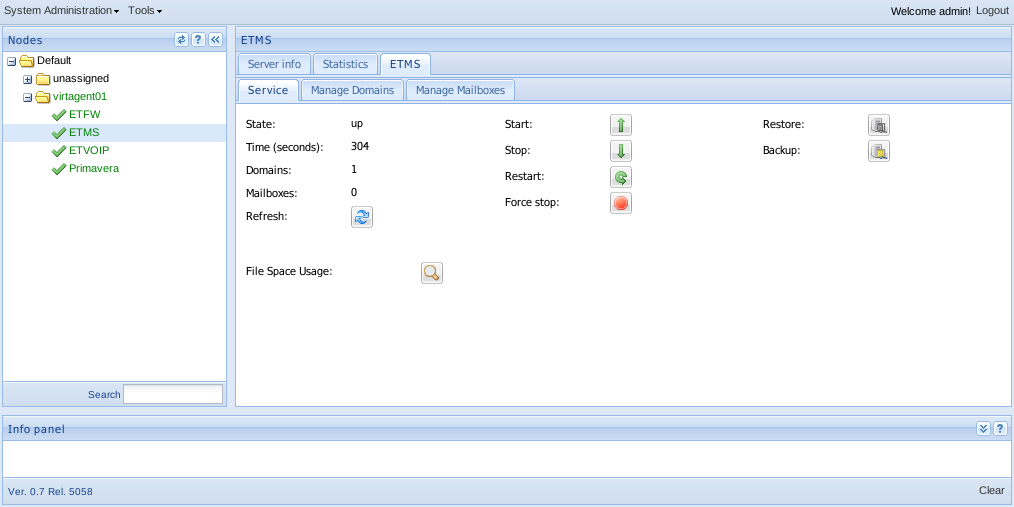
\includegraphics[scale=0.45]{screenshots/etms/etms_main_info.png}
    \caption{ETMS - Main information panel}
    \label{fig:etms_main_info}
    \end{center}
\end{figure}


\subsection{Tab 1 - Service}
\label{sec:etms_info_principal}

The separator \textit{service} is divided into three columns (Figure \ref{fig:etms_main_info}). 
On the left we can see some information about the running process of the service including: information about its state (\textit{Up} - working, \textit{Down} - stopped), the number of domains and email accounts, and the total space occupied by emails on the server. 
Note that the total space occupied is not visible immediately after the opening of the tab, because it is a potentially lengthy operation. 
Thus, to request this information you must select the icon on the right. 
Information on the service status is updated the first time the tab is open and can be refreshed when requested explicitly, through the button \textit{Update}.

In the center column are options for \textit{Start}, \textit{Stop} and \textit{Restart} the process that supports the service. If you are have problems stopping the service, try using the \textit{force stop} button instead the normal one.

In the right column are defined operations for backup and restore settings. These options should only be used to test new settings, because its storage is done locally (on the machine where the mail server).

\subsection{Tab 2 - Manage domains}
\label{sec:etms_gerir_dominios}

The contents of the separator \textit{Manage Domains} is divided into two main areas/grills, where you can select lines (Figure \ref{fig:etms_criar_dominio_1}). The grid on the left lists any existing domains. The right grid, lists the existing alias for the selected domain.

In both areas it is possible to perform operations over the selected items by using the buttons available on the toolbar under the grill in question. Note that selecting a domain, the list of alias gets refreshed.

\begin{figure}[H]
    \begin{center}
    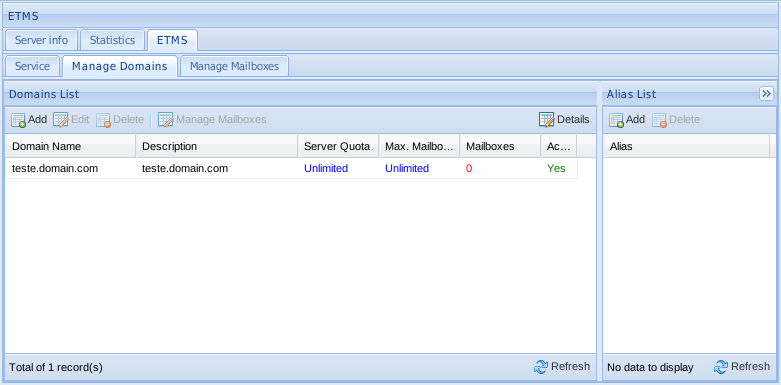
\includegraphics[scale=0.45]{screenshots/etms/etms_criar_dominio_1.png}
    \caption{ETMS - Manage domains panel}
    \label{fig:etms_criar_dominio_1}
    \end{center}
\end{figure}

\subsubsection{Add a new domain}
\label{sec:etms_sub_criacao_dominio}
To create a domain use the \textit{Add domain} button, which opens a window with some fields to fill, as shown in Figure \ref{fig:etms_criar_dominio_2}. After filling the fields press the button \textit{Save} to make the changes. Please note that the first three fields are mandatory; the grid with existing domains is refreshed after adding a new domain.

\begin{figure}[H]
    \begin{center}
    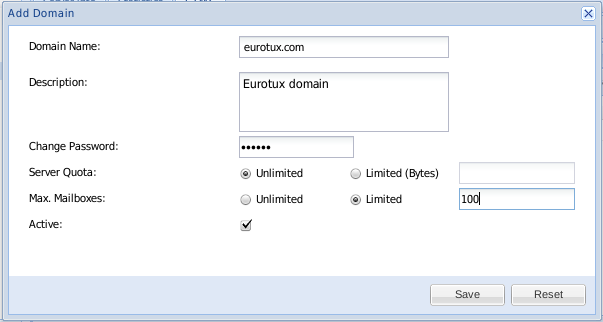
\includegraphics[scale=0.6]{screenshots/etms/etms_criar_dominio_2.png}
    \caption{Add domain}
    \label{fig:etms_criar_dominio_2}
    \end{center}
\end{figure}

For a better understanding, we describe briefly the existing fields, indicating for each example:
\begin{itemize}
\item \textbf{Domain name} - Desired domain name (E.g.: eurotux.com)
\item \textbf{Description} - Short description about the domain (E.g.: IT department)
\item \textbf{Password} - \textit{Password} to use for webmin login, bigger than 6 characters. (E.g.: PassWord)
\item \textbf{Server quota} - Maximum value in Byte for storing email (E.g.: 1000000000 Bytes)
\item \textbf{Number of mailboxes} - Maximum number of mailboxes that can be created in this domain. The reduction of the number of mailboxes (available in option \textit{Edit domain}) will not remove any existing mailboxes. (E.g.: 10)
\item \textbf{Active} Activate or not the domain. This option inhibits the delivery of new messages.
\end{itemize}

\subsubsection{Edit domain}
\label{sec:etms_sub_edicao_dominio}
To edit a domain, select the corresponding line and choose the \textbf{Edit domain} button. It will open a window (see Figure \ref{fig:etms_criar_dominio_2}) with the attributes of the domain pre-filled with the settings previously made (in previous Section \ref{sec:etms_sub_criacao_dominio}).

After saving, the grid that lists your existing domains is updated with the new settings.

\subsubsection{Remove a domain}
\label{sec:etms_sub_remocao_dominio}
The removal of a domain also requires the removal of its alias and associated email accounts (including any existing emails). For removal of a domain, select the line that identifies the domain to remove, and choose the option \textbf{Remove}. Then answer yes to the confirmation question, as shown in Figure \ref{fig:etms_delete_domain}. The success of the operation is shown in \textit{Information Panel}.

\begin{figure}[H]
    \begin{center}
    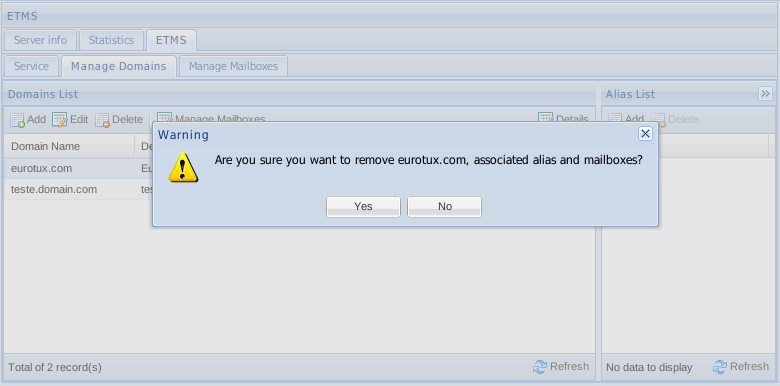
\includegraphics[scale=0.45]{screenshots/etms/etms_delete_domain.png}
    \caption{Remove domain}
    \label{fig:etms_delete_domain}
    \end{center}
\end{figure}


\subsubsection{Manage domain's mailboxes}
\label{sec:etms_sub_gerir_caixas_dominio}
The \textit{Manage Mailboxes} button allows to edit mailboxes. When selected, this option changes the selected tab into \textit{Manage Mailboxes} one. Then a search by domain name is performed (see Figure \ref{fig:etms_gerir_mailboxes}). Note that the \textit{Manage Mailboxes} is only visible if a domain is selected.

\begin{figure}[H]
    \begin{center}
    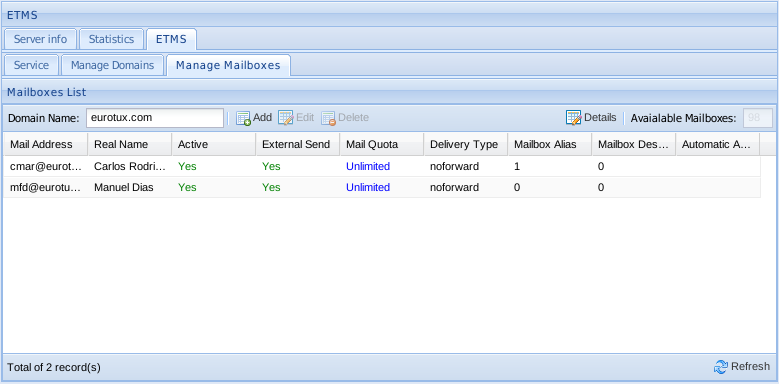
\includegraphics[scale=0.45]{screenshots/etms/etms_gerir_mailboxes.png}
    \caption{Manage domain mailboxes}
    \label{fig:etms_gerir_mailboxes}
    \end{center}
\end{figure}

\subsubsection{Details option}
\label{sec:etms_sub_detalhes_dominio}
The option \textit{Details}, belongs to the toolbar that is under the domains List (at right). Selecting this option is added a column to the grid that lists some information about the occupied space by each domain (see Figure \ref{fig:etms_domain_details}). Note that, because it could be a computational intensive operation this column is only showed on demand. So, whenever you want to update/view the disk space in use, you should use this option.

\begin{figure}[H]
    \begin{center}
    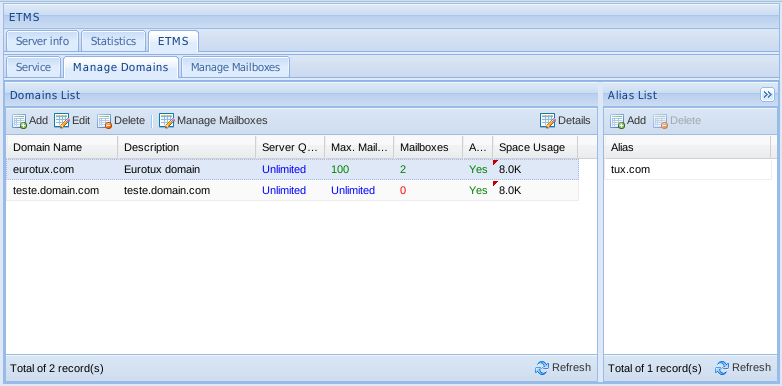
\includegraphics[scale=0.45]{screenshots/etms/etms_domain_details.png}
    \caption{Domains' needed space}
    \label{fig:etms_domain_details}
    \end{center}
\end{figure}

\subsubsection{Adding alias}
\label{sec:etms_sub_criacao_alias_dominio}
To add an \textit{alias}, select the desired domain. In the right area where you can see the alias list, press the \textit{Add} button. Note that an entry is added to the top of the list where you can set the new alias name (see Figure \ref{fig:etms_criar_alias_dominio}). After editing the row, the new \textit{alias} is sent to the service agent. If the operation was successfully accomplished, a notification is displayed (Figure \ref{fig:etms_criar_alias_dominio_success}], and added an entry to the information panel.

\begin{figure}[H]
    \begin{center}
    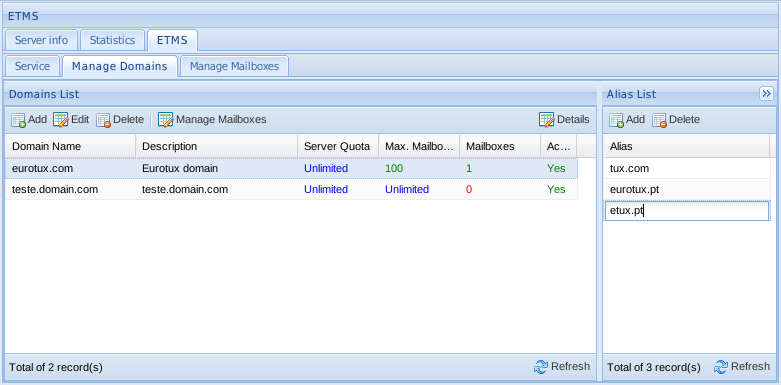
\includegraphics[scale=0.45]{screenshots/etms/etms_criar_alias_dominio.png}
    \caption{Adding a domain alias}
    \label{fig:etms_criar_alias_dominio}
    \end{center}
\end{figure}

\begin{figure}[H]
    \begin{center}
    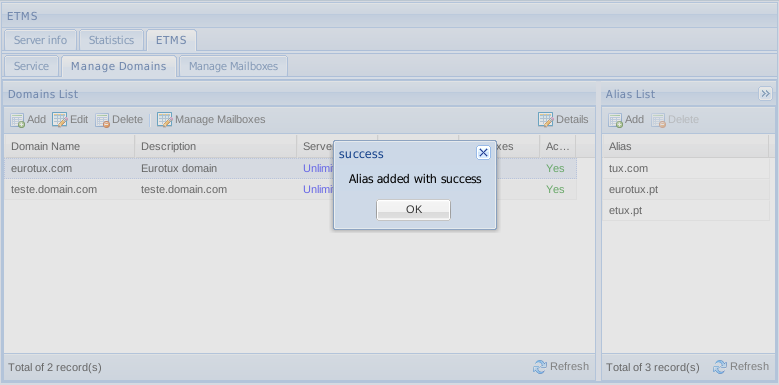
\includegraphics[scale=0.45]{screenshots/etms/etms_criar_alias_dominio_success.png}
    \caption{Alias created successfully}
    \label{fig:etms_criar_alias_dominio_success}
    \end{center}
\end{figure}


\subsubsection{Removing domain's alias}
\label{sec:etms_sub_remocao_alias_dominio}
To remove an alias: select the domain that contains the alias (Figure \ref{fig:etms_criar_alias_dominio}); In the alias list, select the alias that you want to remove; Press the \textit{Remove} button; Answer yes to the confirmation message.

Note that, when necessary, the alias list can be updated through the lower toolbar by pressing the refresh button.

\subsection{Tab 3 - Manage mailboxes}
\label{sec:etms_caixas_correio}
The Manage Mailboxes' tab is an area/grid where each row corresponds to a mailbox (see Figure \ref{fig:etms_gerir_mailboxes_mb}). The grid lines are selectable and can perform operations on each selection. To see the mailboxes it's necessary to perform a search of mailboxes, that can be done by following the steps given in Section \ref{sec:etms_sub_pesquisar_caixas_correio}.

\begin{figure}[H]
    \begin{center}
    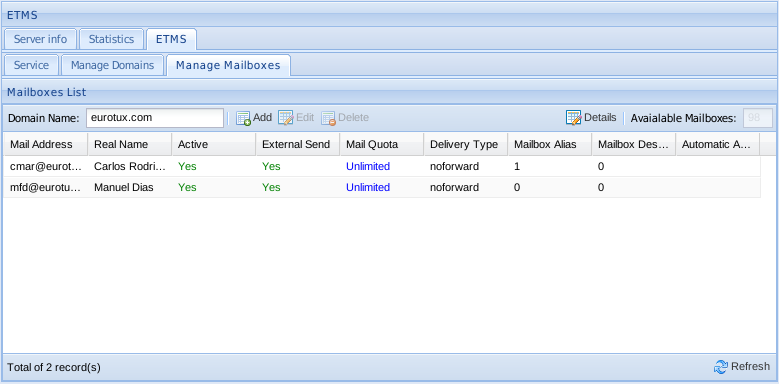
\includegraphics[scale=0.4]{screenshots/etms/etms_gerir_mailboxes.png}
    \caption{ETMS - Mailbox management panel}
    \label{fig:etms_gerir_mailboxes_mb}
    \end{center}
\end{figure}


\subsubsection{Searching for mailboxes}
\label{sec:etms_sub_pesquisar_caixas_correio}

You can search mailboxes for a particular domain, simply enter the domain's name in the box that is over the grill (on the toolbar), and press \textit{ENTER}. Note that during the process of communication with the machine that hosts the service, the icon on the bottom right gets animated (close to the \textit{Update} button). If the domain is not found, an error message is displayed. The success of a search, enables the options for managing mailboxes (see Figure \ref{fig:etms_gerir_mailboxes_mb}).

\subsubsection{Adding a mailbox}
\label{sec:etms_sub_criar_caixas_correio}
To create a mailbox we need to perform a a search by a domain (see Section \ref{sec:etms_sub_pesquisar_caixas_correio}), then use the \textbf{Add} button (It will open a window with fields to fill, as shown in Figure \ref{fig:etms_criar_mailbox}). Press the \textit{Save} to make the change effective. Please note that: the first three fields are mandatory; the grid with existing domains gets refreshed after the addition of the new domain.

\begin{figure}[H]
    \begin{center}
    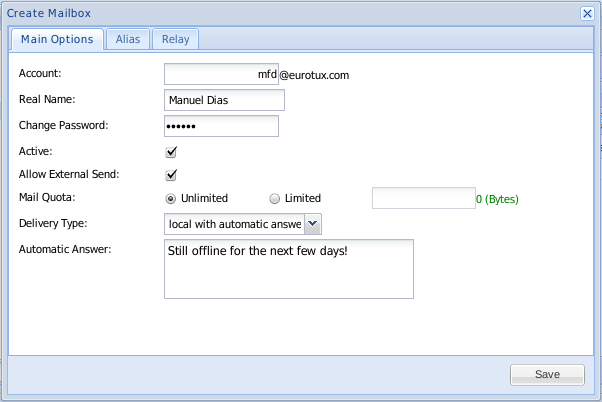
\includegraphics[scale=0.45]{screenshots/etms/etms_criar_mailbox.png}
    \caption{Adding a mailbox}
    \label{fig:etms_criar_mailbox}
    \end{center}
\end{figure}

The window for creating a new mailbox is comprised of three tabs: \textit{Main options}, \textit{Alias} (see Subsection \ref{sec:etms_sub_alias_caixas_correio}), \textit{Forwarding} (see Subsection \ref{sec:etms_sub_encaminhamento_caixas_correio}).

For a better understanding, we describe briefly the existing fields indicating, where appropriate, examples of use:

\begin{itemize}
\item \textbf{Account} - Desired account name(Ex: mfd@eurotux.com)
\item \textbf{Real name} - User name \footnote{I.e. for contacting purposes} (E.g.: Jorge Leal)
\item \textbf{Change password} - \textit{Password} to access into the mailbox. Must be at least six chars long. (E.g.: PassWord)
\item \textbf{Active} - Change the email account's state.
\item \textbf{Allow external send} - Allows the account to send emails off the server that is, domains that are not defined on the server.
\item \textbf{Email quota} - Maximum value to be used for mail storage. Note that at the right, the green indicates the maximum value defined for the domain, and the mail quota cannot exceed this value (e.g. 10000 bytes).
\item \textbf{Delivery type} - There are four modes of delivery: local, forwarded, local and forwarded, forwarded with automatic answer.
\item \textbf{Automatic answer} - Automatic answer message.
\end{itemize}

Here is a list with the various delivery types:
\textit{Local} - Only made mail delivery in the local account, considering also the any existing alias.
\textit{Forwarded} - Only delivers email in the mailboxes defined on tab \textit{Forwarding}.
\textit{Local and forwarded} - The incoming emails are delivered to the local mailbox and sent to mailboxes defined in tab \textit{Forwarding}.
\textit{Local and forwarded with automatic answer} - Emails are delivered in the local mailbox, and a message is sent back to the origin of the email, with text set in \textit{Automatic answer} field.

\subsubsection{Edit a mailbox}
\label{sec:etms_sub_editar_caixas_correio}
The window for editing a mailbox is similar to create mailbox window, described on Section \ref{sec:etms_sub_criar_caixas_correio}. The main difference is that you must select the desired mailbox to change, and choose the option \textit{Edit}. The mailbox form is automatically populated with the account settings and the field\textit {Change Password} is disabled by default. To change the password follow the steps described on Section \ref{sec:etms_sub_password_caixas_correio}.


\subsubsection{Change password}
\label{sec:etms_sub_password_caixas_correio}
To change the \textit{password} of a given account is necessary: select in the grid the desired account, then press edit. In the field \textit{Change Password} select the box that follows it and set the new password. Finally press the save button to complete the configuration (see Figure \ref{fig:etms_mb_pass_ed}).

\begin{figure}[H]
    \begin{center}
    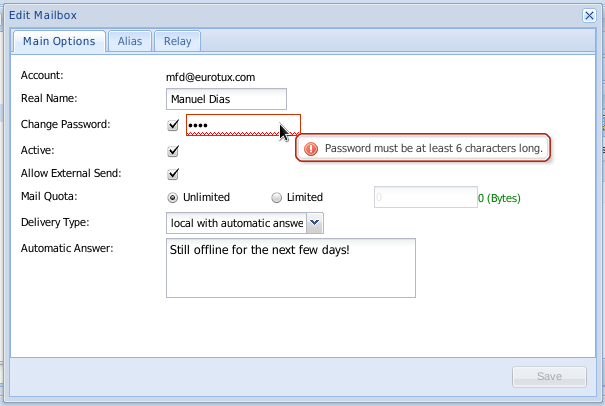
\includegraphics[scale=0.45]{screenshots/etms/etms_mb_pass_ed.png}
    \caption{Change mailbox password}
    \label{fig:etms_mb_pass_ed}
    \end{center}
\end{figure}

\subsubsection{Define mailbox alias}
\label{sec:etms_sub_alias_caixas_correio}
New mailbox alias can be defined to existing mailboxes. Simply add entries in the grid \textit{Alias} in the process of creating/editing a mailbox (described in Section \ref{sec:etms_sub_criar_caixas_correio}). Note that it \textbf{must} be given the full email address (e.g. mfd.alias@eurotux.com), and that the changes take effect after selecting the save option (see figure \ref{fig:etms_alias_create}).

\begin{figure}[H]
    \begin{center}
    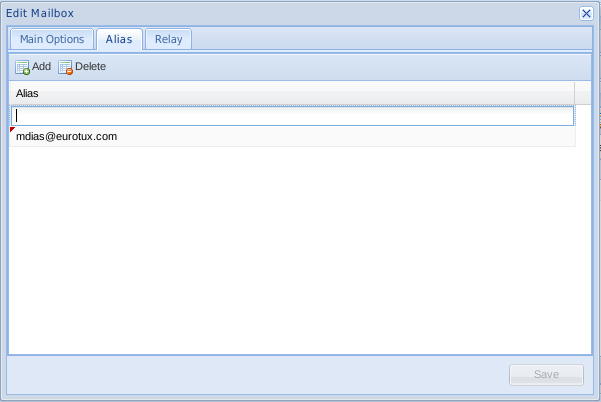
\includegraphics[scale=0.45]{screenshots/etms/etms_alias_create.png}
    \caption{Add mailbox's alias}
    \label{fig:etms_alias_create}
    \end{center}
\end{figure}

To remove alias select the alias you want to remove and choose the option \textit{Remove}. Finally press the save button to make the change effective (see Figure \ref{fig:etms_alias_mailbox_delete} and \ref{fig:etms_alias_mailbox_delete_2}).

\begin{figure}[H]
    \begin{center}
    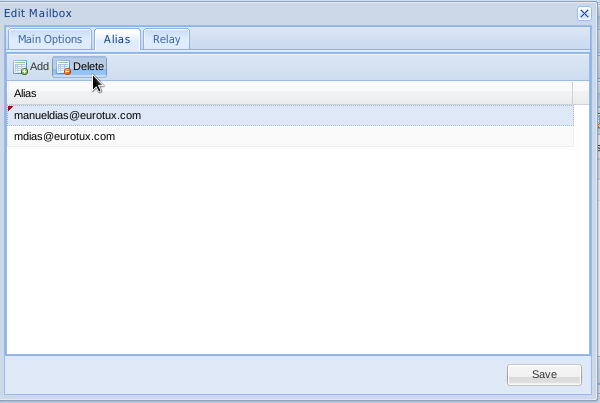
\includegraphics[scale=0.6]{screenshots/etms/etms_alias_mailbox_delete.png}
    \caption{Remove a mailbox alias - step 1}
    \label{fig:etms_alias_mailbox_delete}
    \end{center}
\end{figure}

\begin{figure}[H]
    \begin{center}
    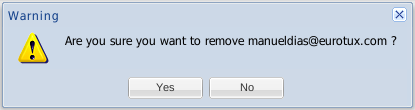
\includegraphics[scale=0.6]{screenshots/etms/etms_alias_mailbox_delete_2.png}
    \caption{Remove a mailbox alias - step 2}
    \label{fig:etms_alias_mailbox_delete_2}
    \end{center}
\end{figure}

\subsubsection{Define forwarding email addresses}
\label{sec:etms_sub_encaminhamento_caixas_correio}
You can define mailboxes into which emails are sent, simply add entries in the grid \textit{Forwarding} in the process of creating/editing, described in \ref{sec:etms_sub_criar_caixas_correio} of a mailbox. Note that you \textbf{must} give the full email address (e.g. mfd@eurotux.pt). Changes will take effect after press the save button (see Figure \ref{fig:etms_alias_create}).

\begin{figure}[H]
    \begin{center}
    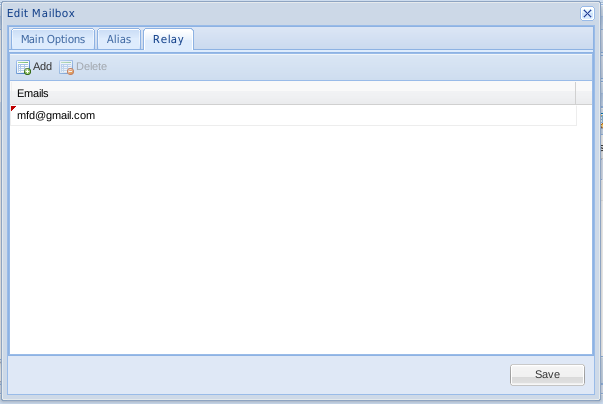
\includegraphics[scale=0.45]{screenshots/etms/etms_forwarding_mb_del.png}
    \caption{Defining forwarding email addresses}
    \label{fig:etms_forwarding_mb_del}
    \end{center}
\end{figure}

The procedure to remove mailboxes is analogous to the removal of domain's alias, simply select the email in question and choose the option \textit{Remove}. Press the save button to changes take effect (analogous to the procedure described in \ref{sec:etms_sub_alias_caixas_correio}).

\subsubsection{Available mailboxes}
\label{sec:etms_sub_disponiveis_caixas_correio}
In the case where the domain has a limited number of mailboxes, the number of available mailboxes appears on the right corner of the tab (see Figure \ref{fig:etms_free_mb}). Every time a mailbox is created, this number is decremented, disabling the option that allows the creation of new mailboxes when the number of mailboxes is equals or exceeds the the domain limit.

\begin{figure}[H]
    \begin{center}
    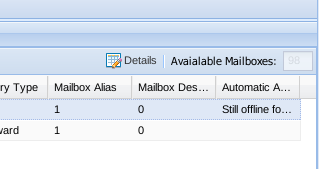
\includegraphics[scale=0.6]{screenshots/etms/etms_free_mb.png}
    \caption{Available mailboxes}
    \label{fig:etms_free_mb}
    \end{center}
\end{figure}

\subsubsection{Details option}
\label{sec:etms_sub_detalhes_caixas_correio}
The details option, belongs to the toolbar that it's under the mailbox's list (at right). When selected, this option append to the grid two columns to the grid that lists mailboxes with information on the space occupied by the messages received (see Figure \ref{fig:etms_mb_space}). Note that, because it can be a computational intensive operation and potentially time-consuming, the columns only appears on request. So, whenever you want to update/view the disk space occupied, it should be used if this option. If new mailboxes are added, the value does not appear, this happens because of the directories that store the emails have not yet been created.

\begin{figure}[H]
    \begin{center}
    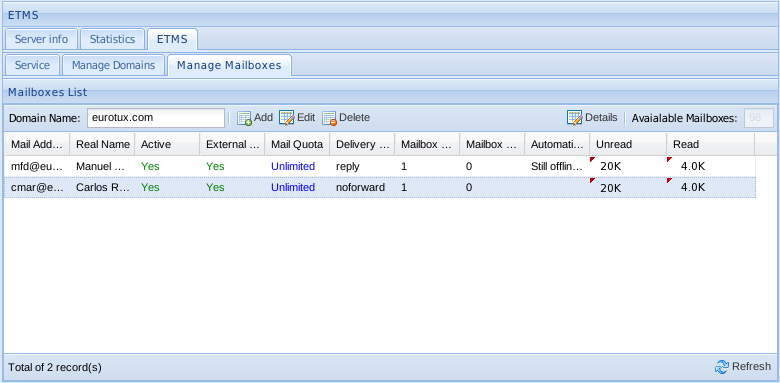
\includegraphics[scale=0.45]{screenshots/etms/etms_mb_space.png}
    \caption{Occupied disk space by mailboxes emails}
    \label{fig:etms_mb_space}
    \end{center}
\end{figure}



\subsubsection{Remove a mailbox}
\label{sec:etms_sub_apagar_caixas_correio}
Removing a mailbox, in addition to removing all settings, deletes all the emails in the selected account (and you can not retrieve them through the process of restoration of settings). To remove an account, search for the desired mailbox \ref{sec:etms_sub_pesquisar_caixas_correio}, choose the corresponding line, press the \textit{Remove} button (Figure \ref{fig:etms_mb_del}).

\begin{figure}[H]
    \begin{center}
    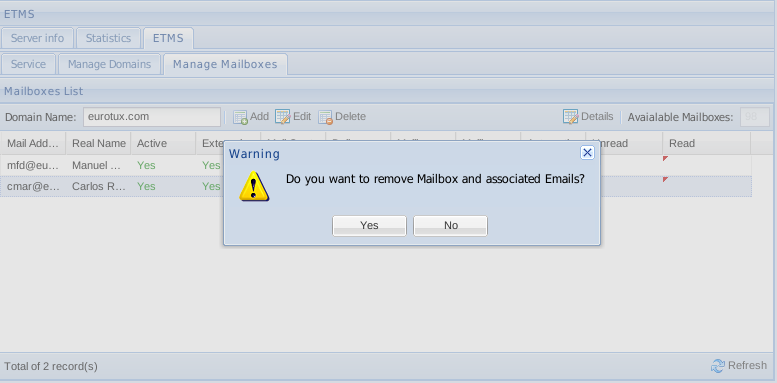
\includegraphics[scale=0.6]{screenshots/etms/etms_mb_del.png}
    \caption{Remove mailbox - confirmation question}
    \label{fig:etms_mb_del}
    \end{center}
\end{figure}
